\documentclass{ctexart}
\usepackage{subfigure}

\begin{document}
\heiti
\title{周报} 
\author{刘精昌}
\maketitle

\fangsong
\begin{itemize}
  \item 阅读MCMC的一篇introduction的前半部分,《An Introduction to MCMC for Machine Learning》。目前看了拒绝抽样法、重要抽样法、H-M算法、模拟退火等。
  \item 看了毕业设计相关的ppt、数据等,数据的问题是数据比较大、类型不清楚、缺少labels。
  \item 阅读《A Symbolic Representation of Time Series, with Implications for Streaming Algorithms》.SIGMOD 2003 以及《Experiencing SAX: A novel symbolic representation of time series》.DMKD 2007。这两篇文章系同一作者,内容几乎一致。介绍了时间序列的一种符号串表示方法。此方法可以有效地降维以及数值约减,以进一步地进行聚类、分类等操作。主要包括下面两步。
      \begin{enumerate}
        \item 使用Piecewise Aggregate Approximation (PAA)对原数据进行处理。PAA这种技巧很简单,我之前的论文里面看到过,就是对时间序列等分段,每一段的时间序列用均值代替,如图1所示。
        \begin{figure}
          \centering
          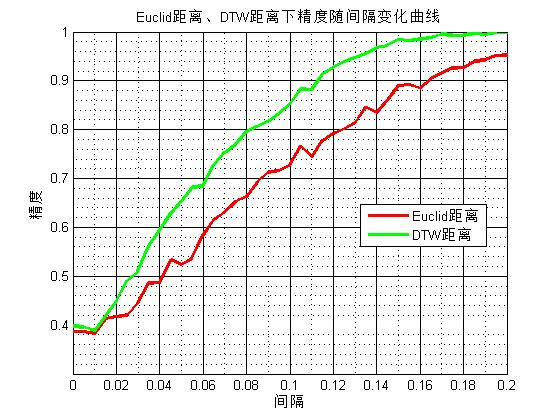
\includegraphics[width=0.6\textwidth]{1.jpg}
          \caption{PAA示意图}\label{figure:a}
        \end{figure}
            
        \item 对PAA处理后的时间序列进行字符化。首先假定时间序列数据满足正态分布,然后对正态分布的CDF等概率划分,把每一概率对应的时间序列区段映射到相应的字符上,如图2所示。
        \begin{figure}
          \centering
          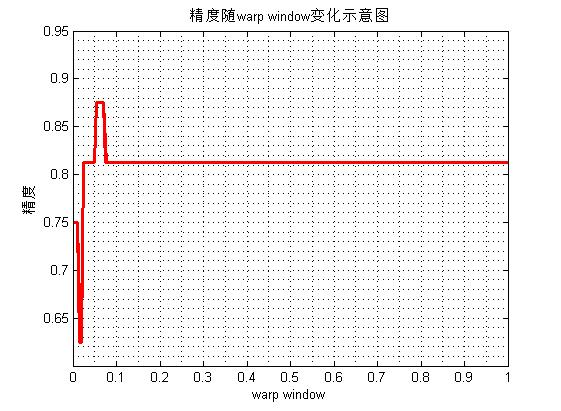
\includegraphics[width=0.6\textwidth]{2.jpg}
          \caption{离散化示意图}\label{figure:b}
        \end{figure}
        把PAA结果用符号表示可以进一步的约减数据,因为一连串的相同字符可以用数字表示次数,而不需要将每一个字符都写下来。
      \end{enumerate}
      本文指出,把时间序列用符号串表示出来后,可以进一步地利用符号处理的相关方法,比如suffix tree对符号串处理,以完成进一步的任务,比如:聚类、分类。
\end{itemize}

\end{document}